\chapter{ТУРШИЛТ БА ҮР ДҮН}
Энэ бүлэгт илрүүлэгчийн сургалт, уншигчийн үе шаттай сургалт, тэмдэгтийн андуурлын шинжилгээ, төгсгөл хүртэлх ба олон кадрын үр дүн, хугацааны хэмжилт, бичлэгийн туршилтын үр дүнг үзүүлнэ. Бүх хэмжилт 2026 оны 10 дугаар сарын 14-ний сургалтын жингээр, \texttt{scripts/eval\_pipeline.py} скриптээр хийгдсэн; тоонуудыг \texttt{runs/eval/results.json}-д хадгалсан.

\section{Дугаар илрүүлэгчийн үр дүн}
Зураг~\ref{fig:detcurves}-д хоёр үе шатны сургалтын муруйг үзүүлэв. A үед ерөнхий шалгалтын mAP$_{50}$ эхний эпохоос 0.95-аас дээш гарч 25 эпохын эцэст 0.981 болсон нь дугаарын геометр улс орноос үл хамааран ижил гэдгийг илтгэнэ. B үед монгол зураг нэмэгдсэнээр монгол шалгалтын mAP$_{50\text{--}95}$ 0.69-өөс 0.83 хүртэл өссөн бол mAP$_{50}$ 0.99 орчимд тогтвортой байв: нарийн тохируулга дугаарыг \emph{олох} бус \emph{хайрцгийг нарийн тавих} чадварыг сайжруулсан бөгөөд энэ нь хоёр мөрт дугаарын мөр хуваалтад чухал. Сургалтын алдагдал B үеийн эхэнд (шинэ өгөгдөл) бага зэрэг өсөөд тогтмол буурсан; шалгалтын алдагдал 25 эпохоос хойш хэлбэлзэлтэй ч өсөөгүй тул хэт тохирол ажиглагдсангүй. Хүснэгт~\ref{tab:det}-д сургалт, шалгалт, тестийн олонлог тус бүрийн үр дүнг үзүүлэв; ерөнхий тест (882 зураг) ба шалгалт (1\,765) ойролцоо байгаа нь монгол зургаар тохируулахад ерөнхий чадвар алдагдаагүйг харуулна.
\begin{figure}[H]\centering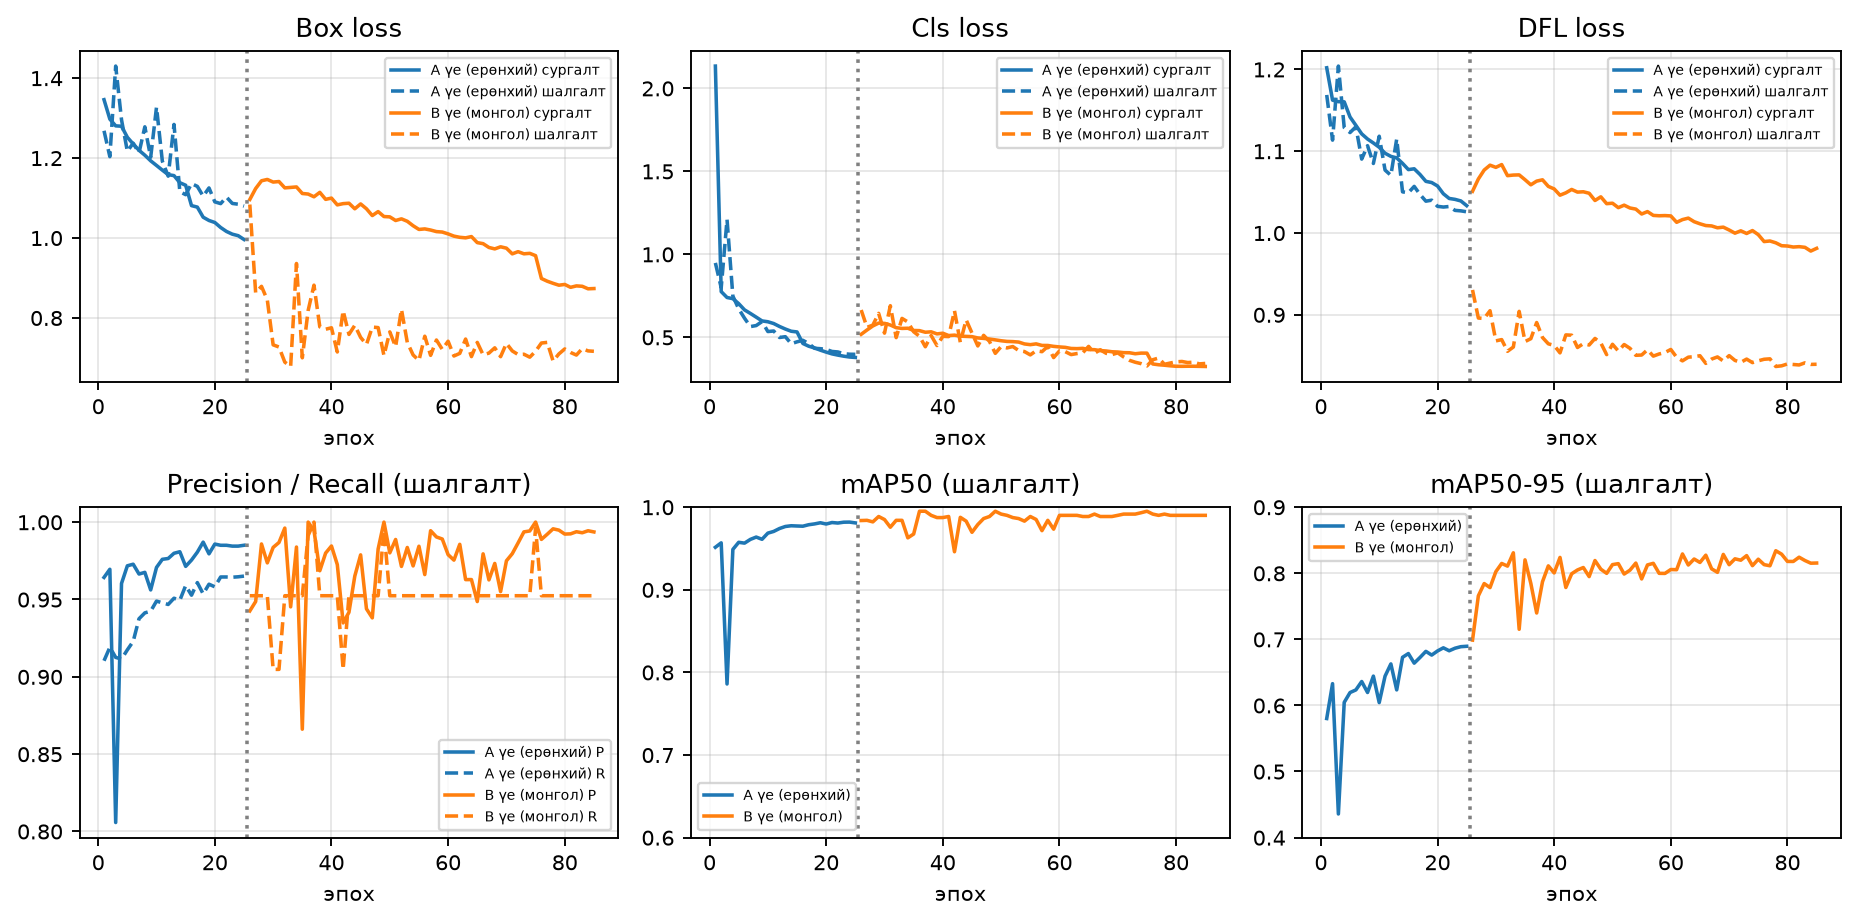
\includegraphics[width=\textwidth]{det_curves.png}
\caption{YOLO11n илрүүлэгчийн сургалтын муруй: box, cls, DFL алдагдал (сургалт --- бүтэн, шалгалт --- тасархай), precision/recall, mAP$_{50}$, mAP$_{50\text{--}95}$ эпох бүрээр. Босоо тасархай шугам A үеэс (ерөнхий 8\,823 зураг) B үе (монгол нэмсэн) рүү шилжсэн цэг; B үеийн шалгалт монгол 18 зураг.}\label{fig:detcurves}\end{figure}
\begin{table}[H]\centering\caption{YOLO11n илрүүлэгчийн үр дүн, 640~px, эцсийн жин (B үеийн 53 дахь эпох)}\label{tab:det}
\resizebox{\textwidth}{!}{\begin{tabular}{lrcccc}\toprule
Олонлог & Зураг & P & R & mAP$_{50}$ & mAP$_{50\text{--}95}$\\\midrule
Монгол шалгалт (GitHub) & 18 (21 дугаар) & 0.996 & 0.952 & \textbf{0.992} & 0.834\\
Ерөнхий шалгалт (HF val) & 1\,765 & 0.974 & 0.970 & 0.982 & 0.699\\
Ерөнхий тест (HF test) & 882 & 0.995 & 0.973 & 0.985 & 0.708\\\bottomrule
\end{tabular}}\end{table}
\begin{figure}[H]\centering
\begin{subfigure}{0.48\textwidth}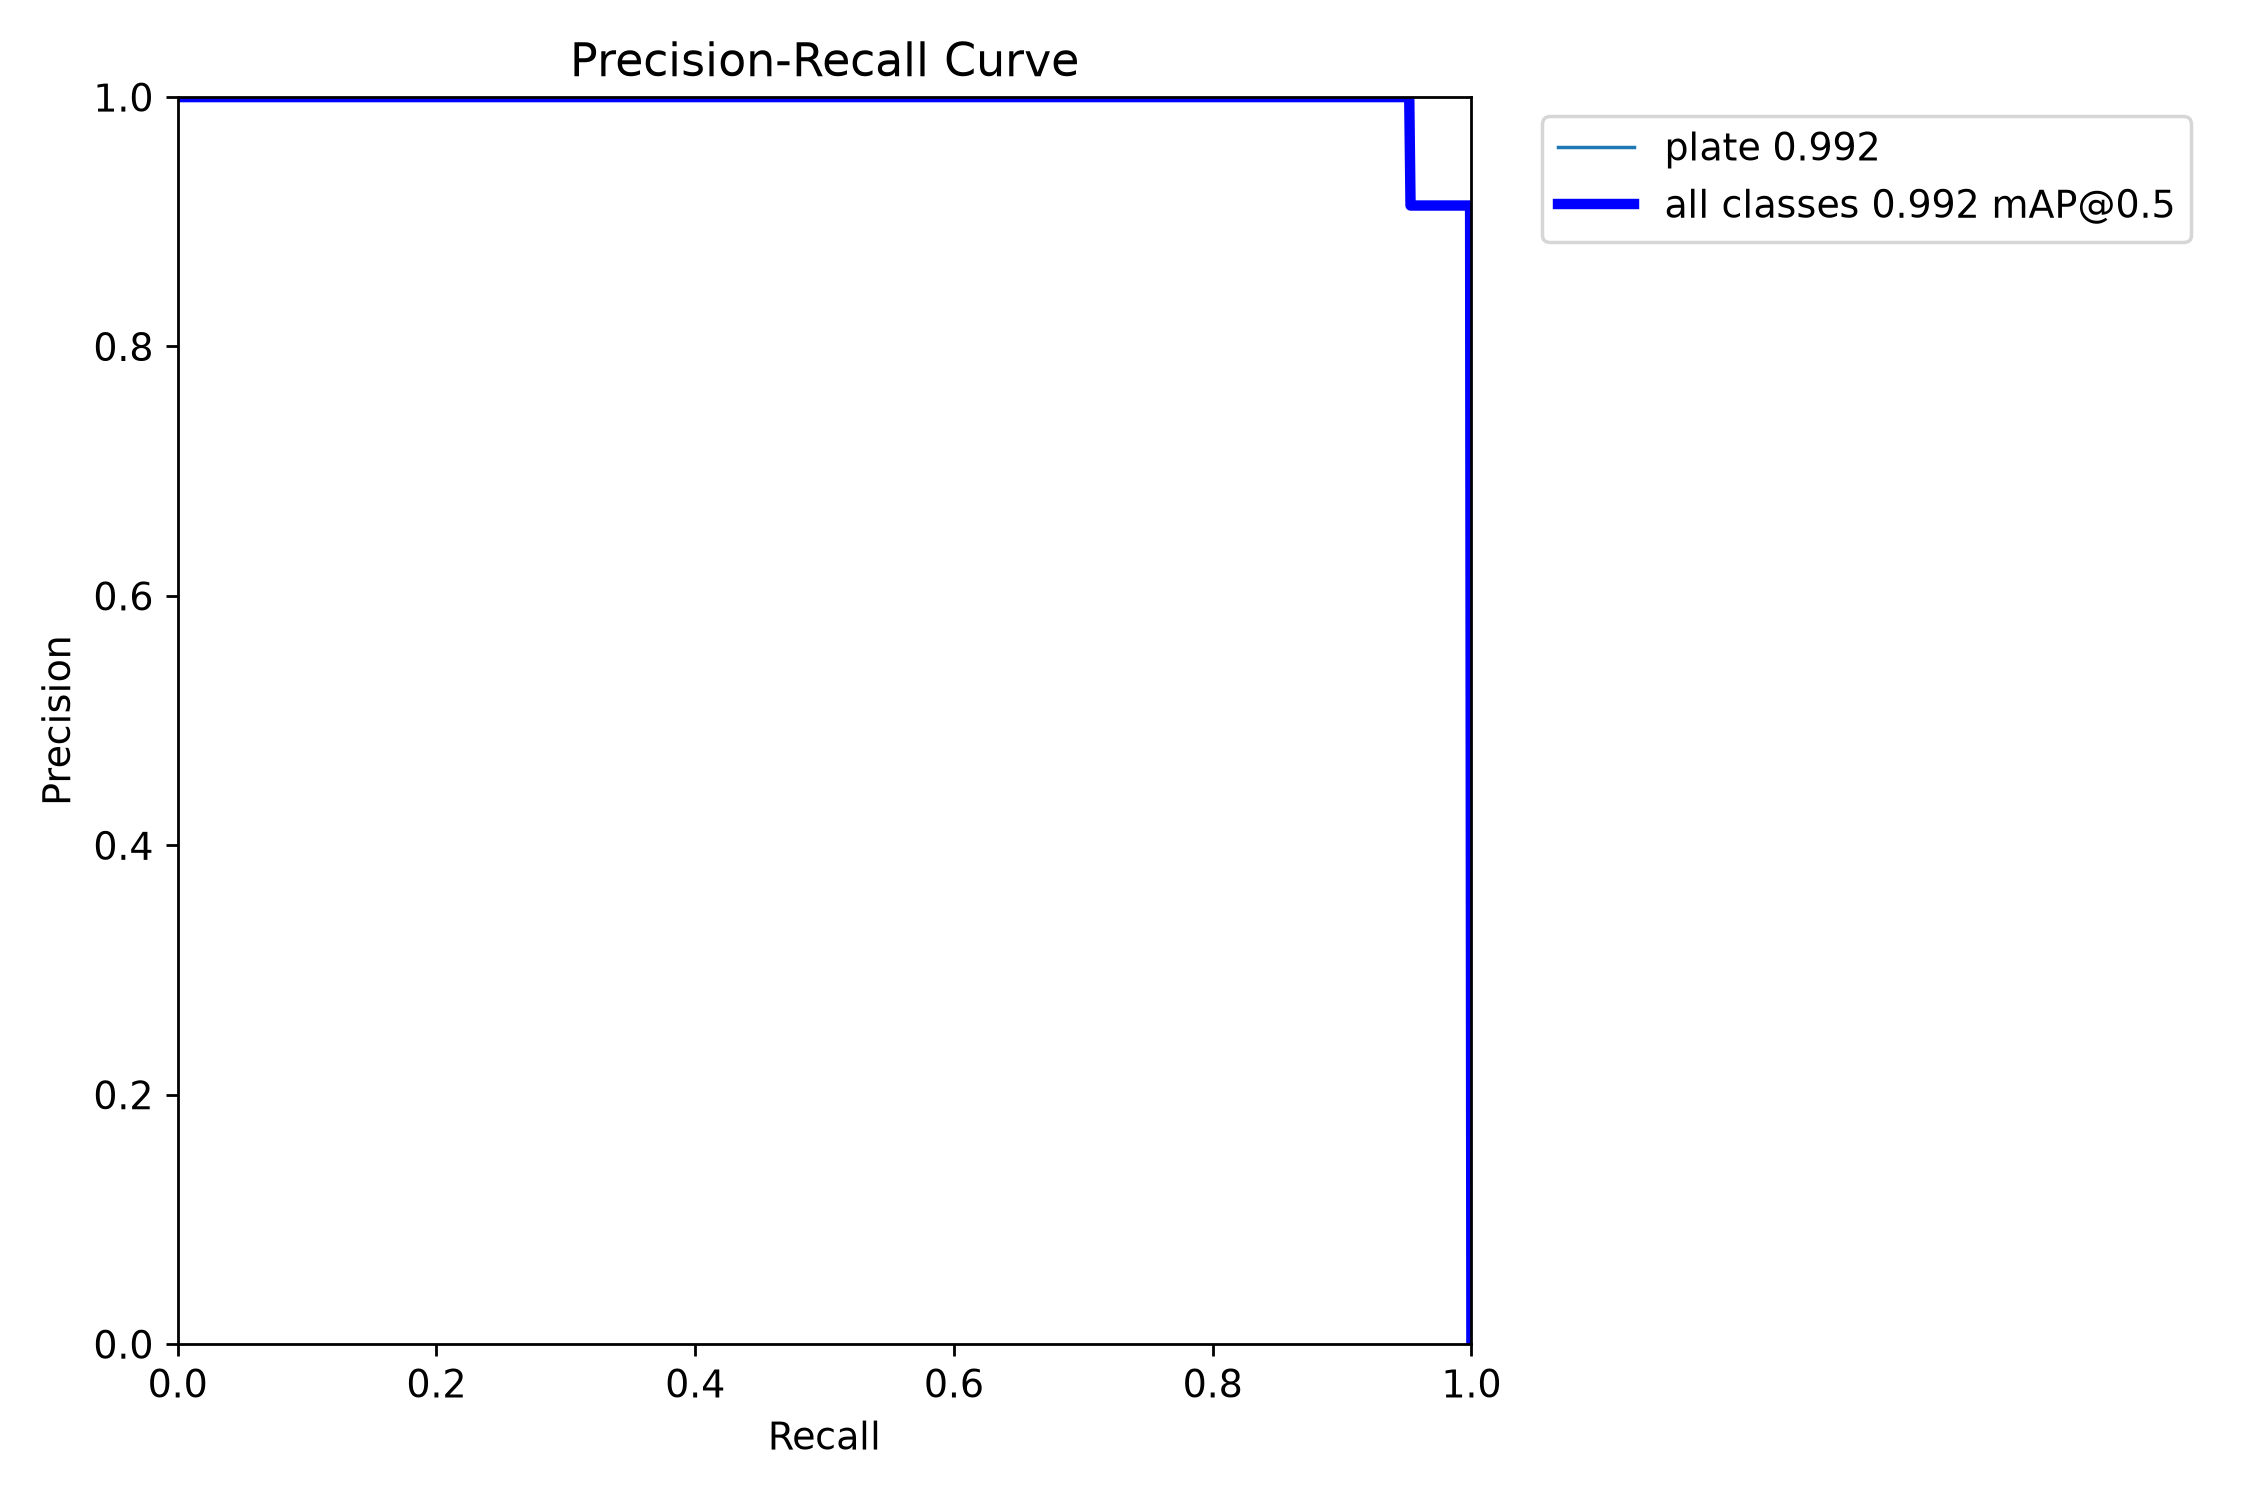
\includegraphics[width=\textwidth]{det_BoxPR_curve.png}\caption{Precision--Recall муруй}\end{subfigure}\hfill
\begin{subfigure}{0.48\textwidth}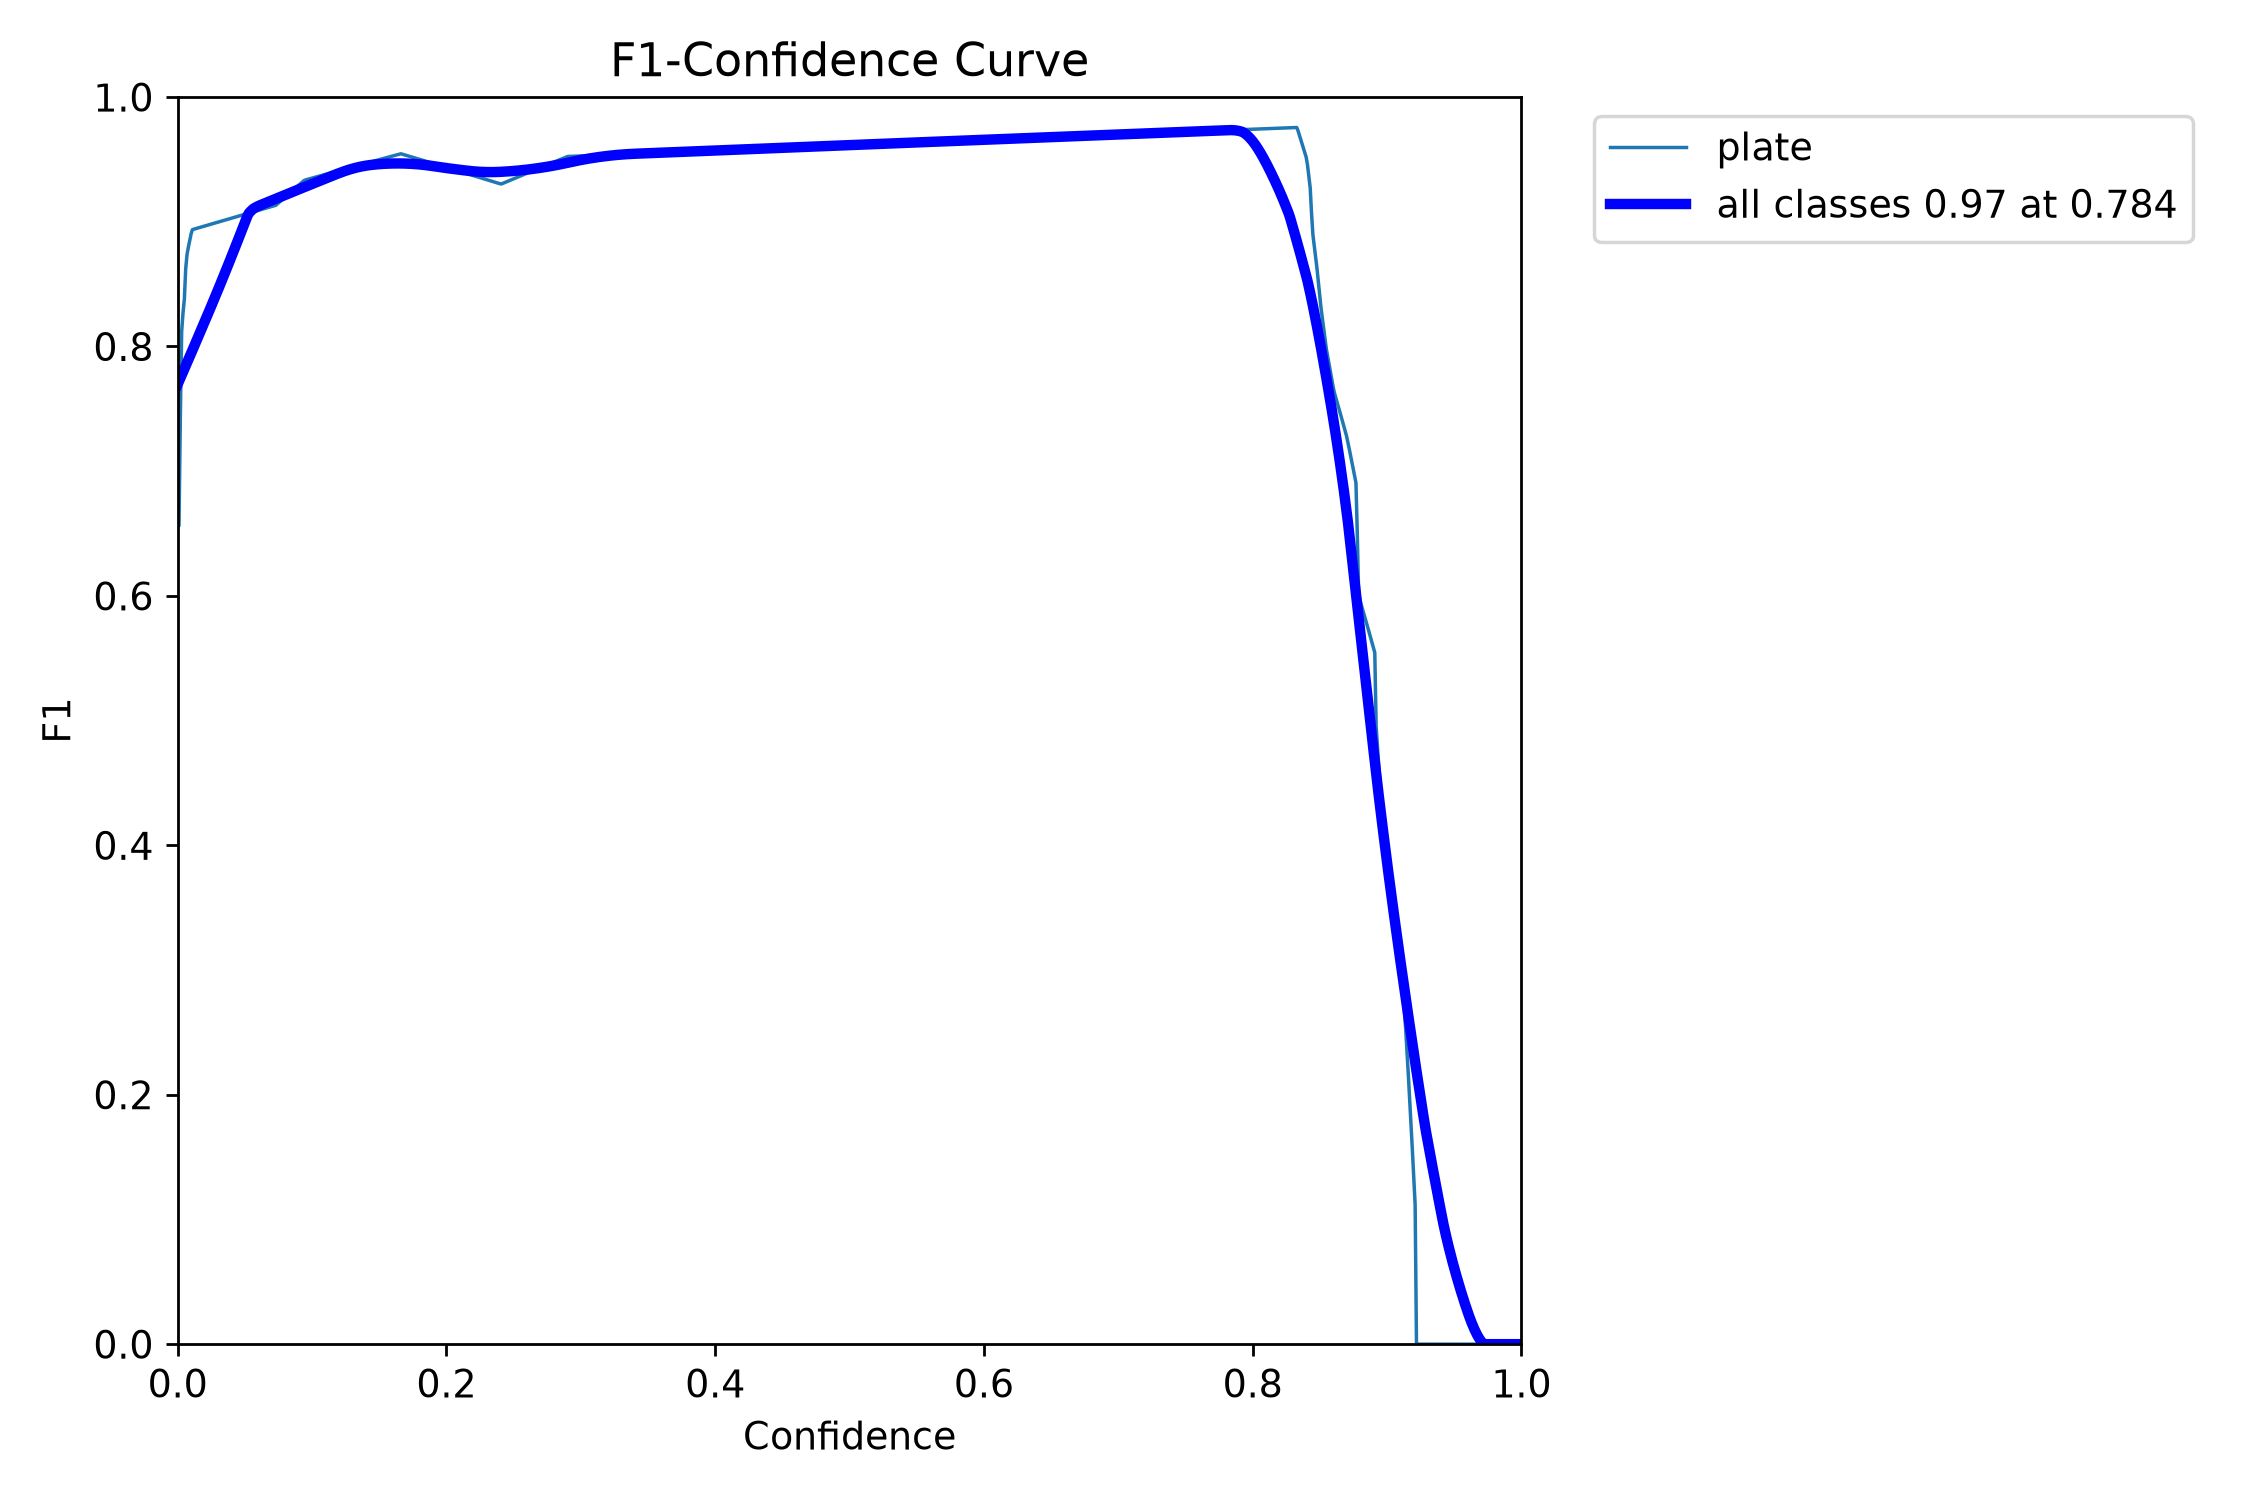
\includegraphics[width=\textwidth]{det_BoxF1_curve.png}\caption{F1--итгэлийн босго муруй}\end{subfigure}
\caption{Илрүүлэгчийн PR ба F1 муруй, монгол шалгалтын олонлог. F1 муруй conf $=0.4$ орчимд хамгийн өндөр байгаа тул урсгалын итгэлийн босгыг 0.4 гэж сонгосон.}\label{fig:detpr}\end{figure}
\begin{figure}[H]\centering
\begin{subfigure}{0.42\textwidth}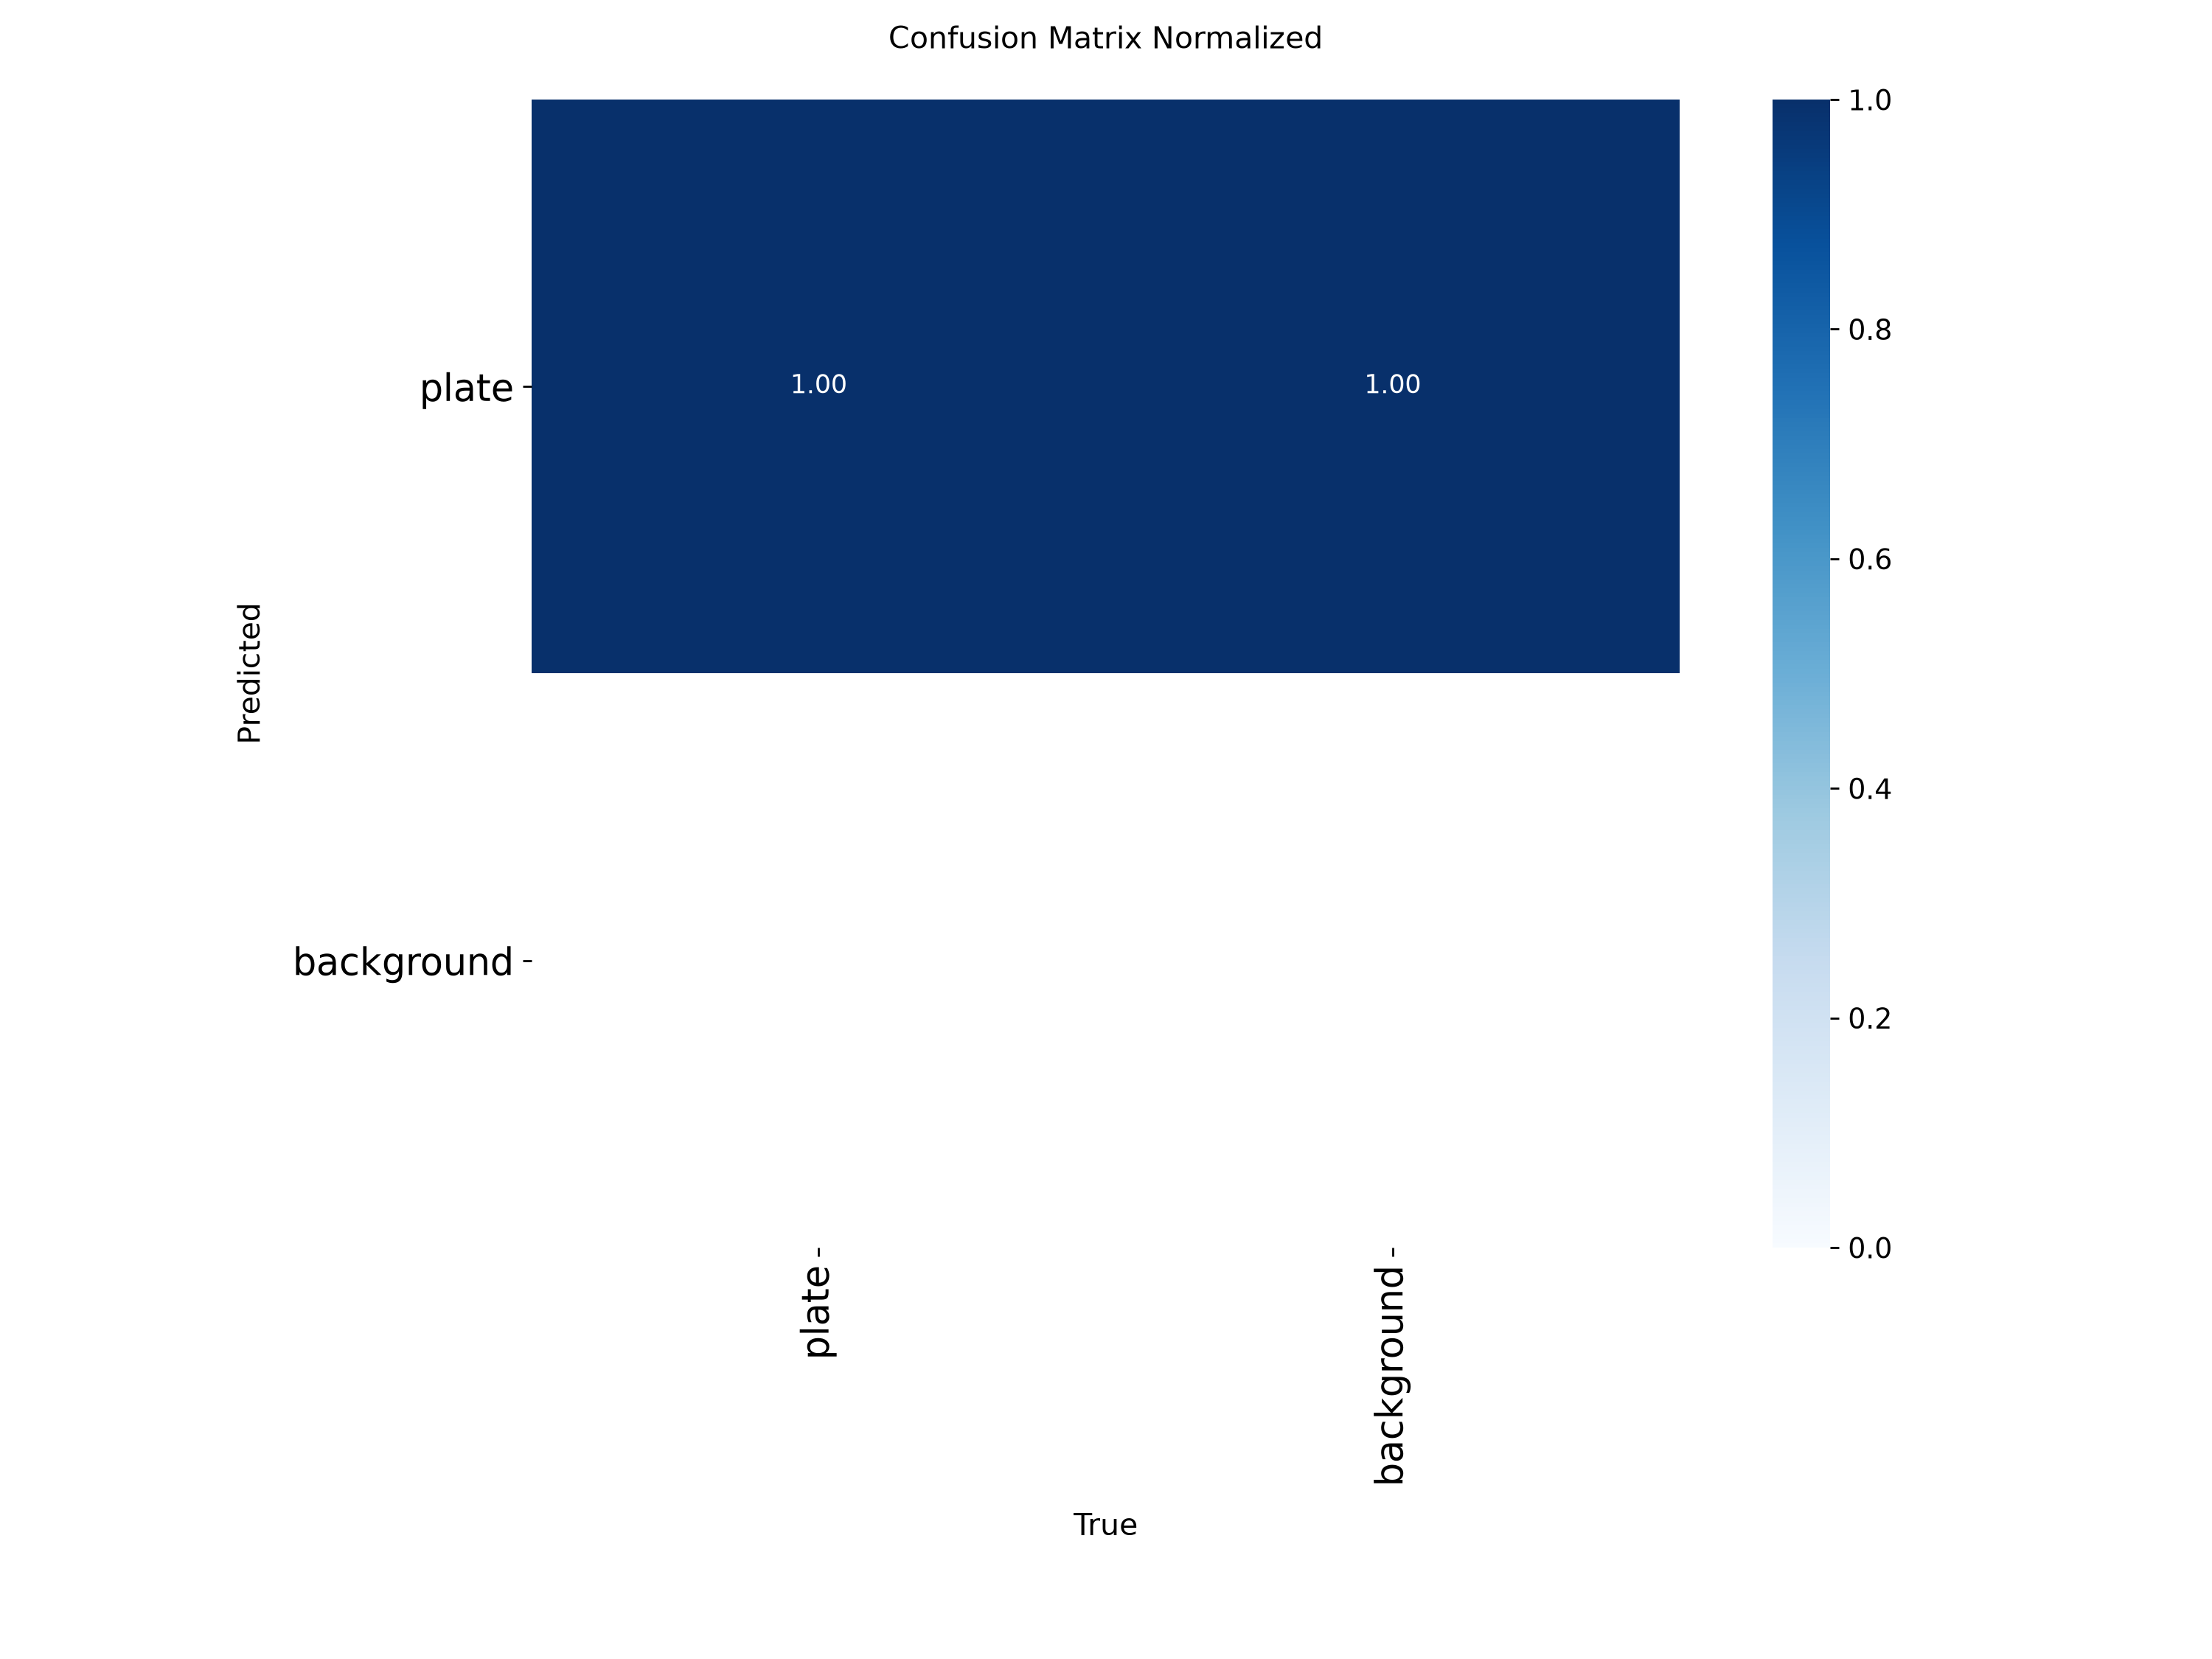
\includegraphics[width=\textwidth]{det_confusion_matrix_normalized.png}\caption{Нормчилсон андуурлын матриц (дугаар / дэвсгэр)}\end{subfigure}\hfill
\begin{subfigure}{0.55\textwidth}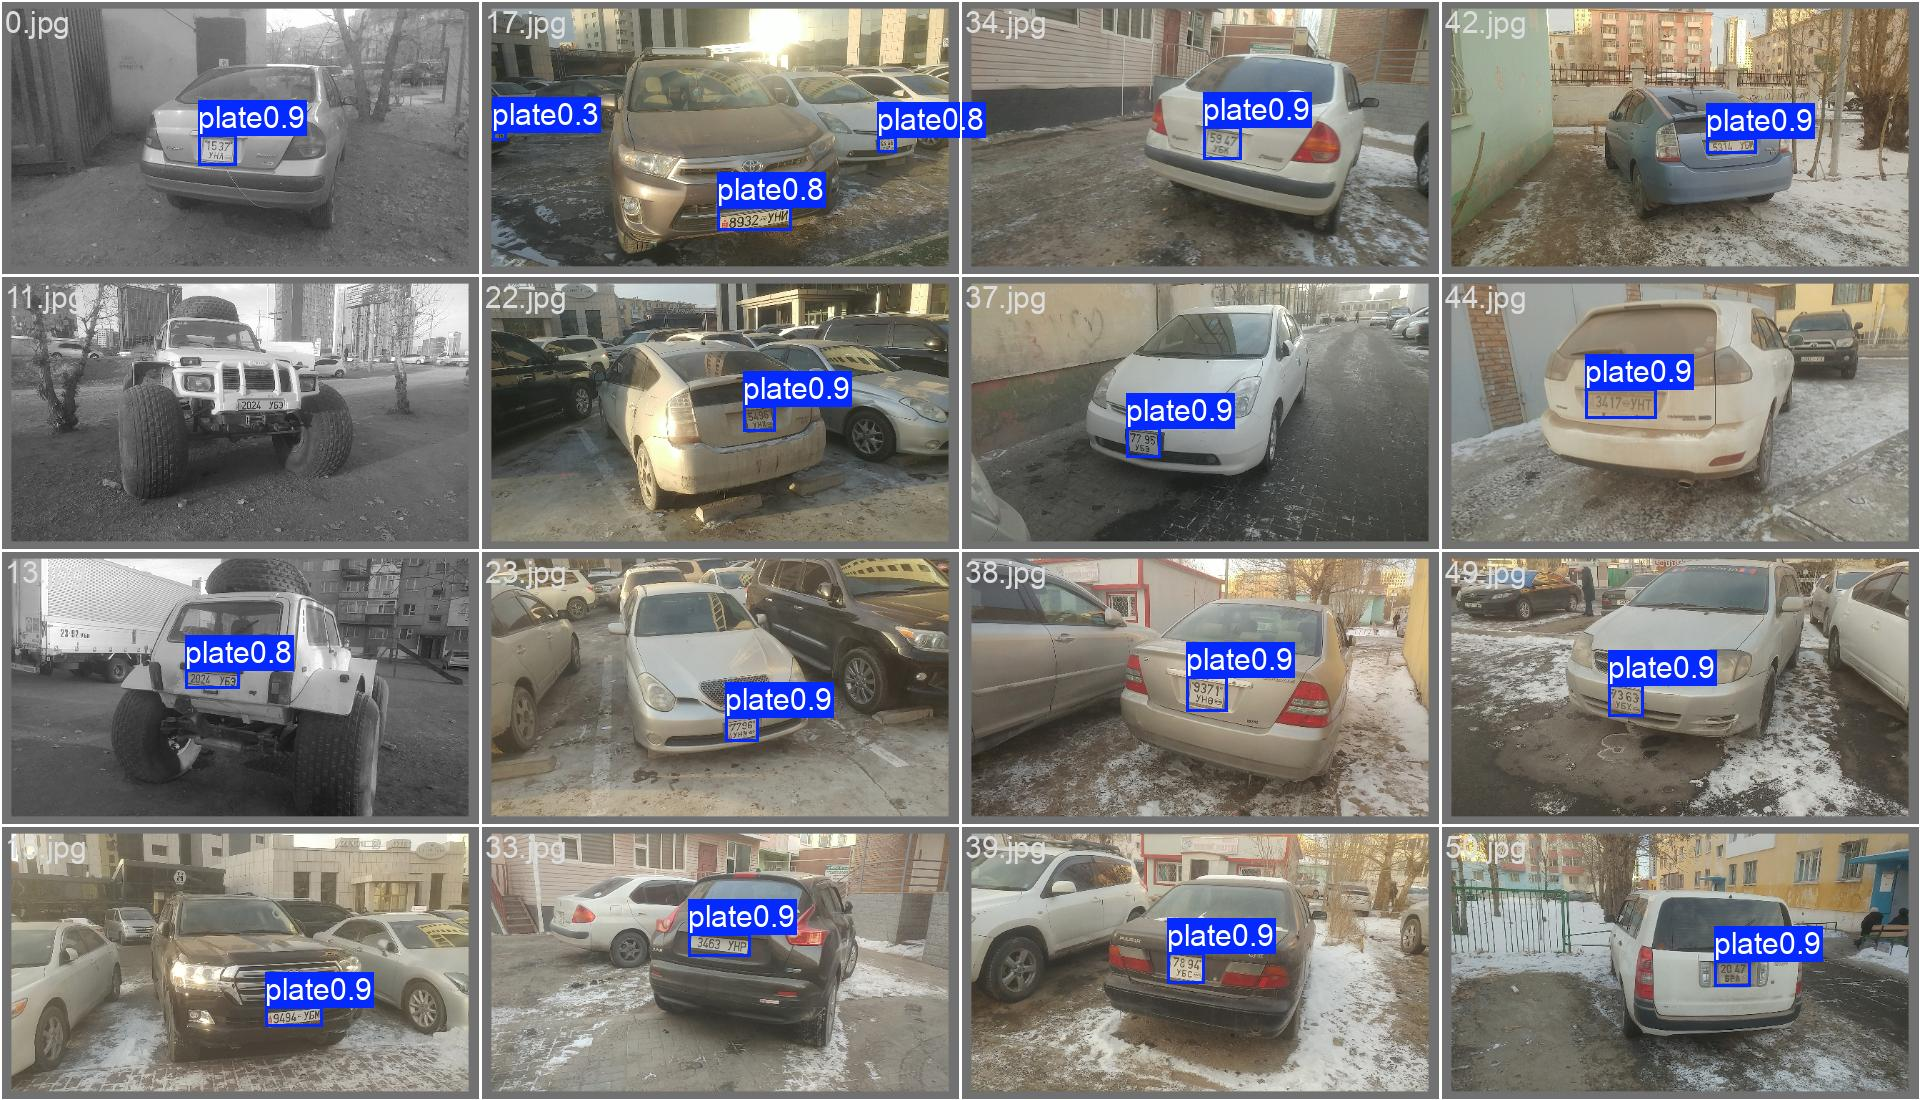
\includegraphics[width=\textwidth]{det_val_batch0_pred.jpg}\caption{Шалгалтын зураг дээрх таамаг}\end{subfigure}
\caption{Илрүүлэгчийн андуурлын матриц ба шалгалтын багцын таамаглал (Ultralytics-ийн гаралт).}\label{fig:detcm}\end{figure}

\section{Уншигчийн сургалтын муруй ба үе шатны нөлөө}
Зураг~\ref{fig:reccurves}-д дөрвөн үе шатны 44 эпохын муруйг үзүүлэв. Зөвхөн синтетикээр (1-р үе) GitHub бодит дугаар дээр 42.1 хувь, CER 0.27 хүрсэн нь рендер дугаарын дизайныг зөв дуурайсан ч бодит камерын шуугиан, бохирдлыг хангалтгүй дуурайж байгааг илтгэнэ. 74 бодит мөр нэмэхэд (2-р үе) эхний эпохдоо 84.2 хувь болж, CER 0.02 хүртэл буурсан --- цөөн ч гэсэн бодит өгөгдөл домэйн зөрүүг ихээхэн хаасан. MLUB нэмсэн 3-р үед шалгалт MLUB-ийн 1\,491 дугаар болж 8 эпохын дараа 91.9 хувь, хэлбэрийн шошгыг засч 20 эпох сургасны дараа 96.8 хувь, CER 0.0064-д хүрсэн. GitHub дугаар дээрх нарийвчлал 3-р үед 84--95 хувийн хооронд хэлбэлзсэн нь 19 дугаарын тест нэг дугаар = 5.3 нэгж хувь гэсэн мөхлөгтэй учир юм. Хүснэгт~\ref{tab:ablation}, Зураг~\ref{fig:ablation}-д үе шат тус бүрийн хамгийн сайн үр дүнг нэгтгэв.
\begin{figure}[H]\centering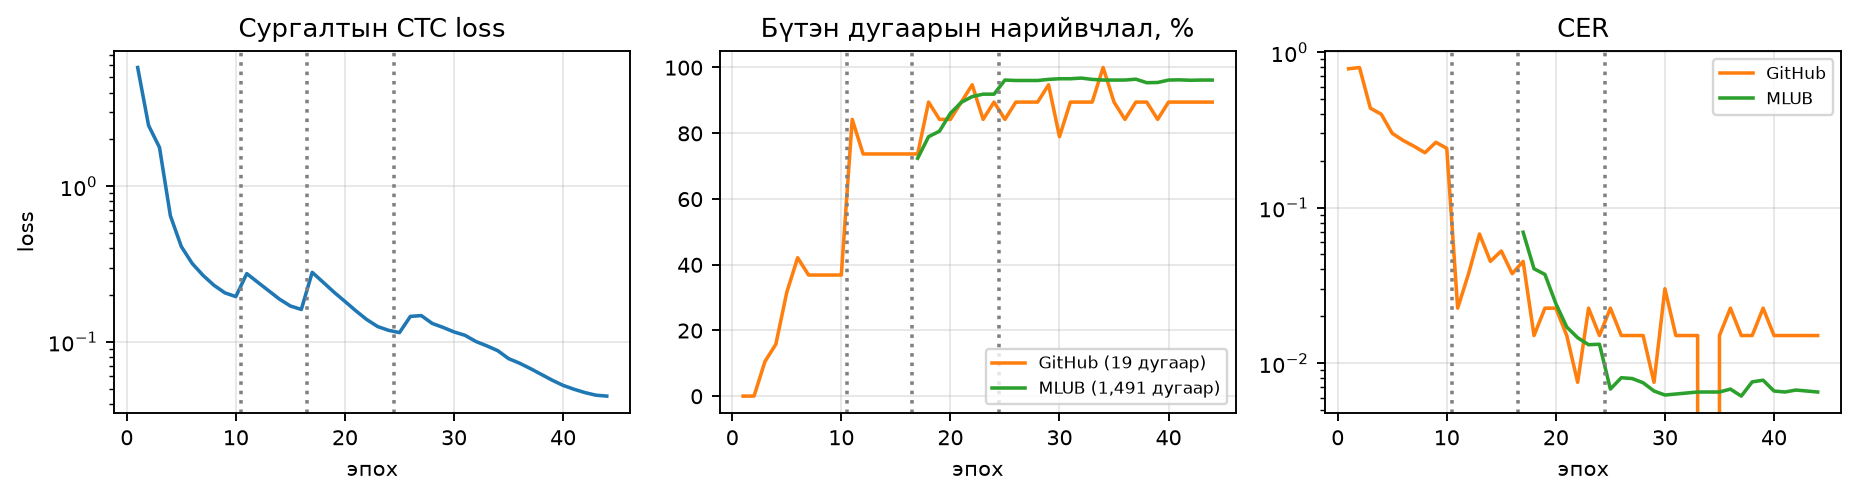
\includegraphics[width=\textwidth]{rec_curves.png}
\caption{CRNN уншигчийн сургалтын муруй, 44 эпох: сургалтын CTC алдагдал (зүүн), бүтэн дугаарын нарийвчлал (дунд), CER (баруун, логарифм). Босоо тасархай шугамууд үе шатны зааг (1: синтетик; 2: +GitHub; 3а: +MLUB; 3б: шошго засч дахин). GitHub муруй 1--2-р үед шалгалт, 3-р үед тест; MLUB муруй 3-р үеийн шалгалт.}\label{fig:reccurves}\end{figure}
\begin{table}[H]\centering\caption{Сургалтын өгөгдлийн нөлөө (ablation): үе шат тус бүрийн хамгийн сайн эпохын үр дүн, бүтэн дугаарын нарийвчлал (хувь) ба CER}\label{tab:ablation}
\resizebox{\textwidth}{!}{\begin{tabular}{lcccc}\toprule
Сургалтын өгөгдөл & GitHub (19), хувь & GitHub CER & MLUB (1\,491), хувь & MLUB CER\\\midrule
Зөвхөн синтетик & 42.1 & 0.271 & --- & ---\\
+ GitHub 74 мөр & 84.2 & 0.023 & --- & ---\\
+ MLUB, анхны шошго (3а) & 84.2 & 0.023 & 91.9 & 0.013\\
+ MLUB, засварласан шошго (3б, эцсийн) & \textbf{89.5} & \textbf{0.015} & \textbf{96.8} & \textbf{0.0064}\\\bottomrule
\end{tabular}}\end{table}
\begin{figure}[H]\centering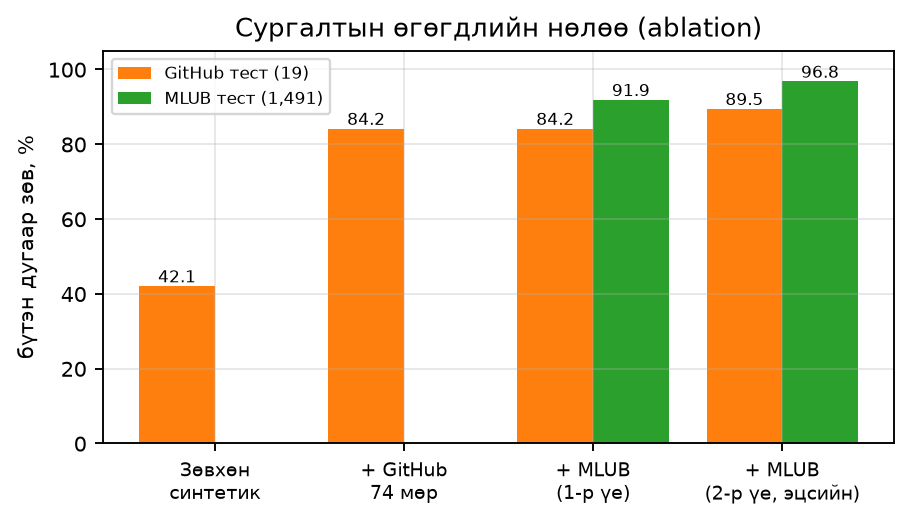
\includegraphics[width=0.7\textwidth]{ablation.png}
\caption{Сургалтын өгөгдлийг шат дараалан нэмэхэд бүтэн дугаарын нарийвчлал хэрхэн өссөн нь.}\label{fig:ablation}\end{figure}

\section{Уншигчийн эцсийн үр дүн}
Хүснэгт~\ref{tab:rec}-д эцсийн уншигчийн үр дүнг олонлог, хэлбэрээр задалж үзүүлэв. MLUB тест дээр хоёр мөрт дугаар (98.4 хувь) нэг мөртөөс (95.8 хувь) өндөр байгаа нь хоёр мөрт дугаарын мөр бүр 3--4 тэмдэгттэй, тэмдэгт бүр илүү том харагддагтай холбоотой.
\begin{table}[H]\centering\caption{Эцсийн CRNN уншигчийн үр дүн, бодит дугаар дээр}\label{tab:rec}
\begin{tabular}{llrcc}\toprule
Нөхцөл & Тест & N & CER & Бүтэн зөв, хувь\\\midrule
Үнэн хайрцгийн тайралт & MLUB & 1\,491 & 0.0065 & \textbf{96.8}\\
\quad нэг мөрт & MLUB & 927 & --- & 95.8\\
\quad хоёр мөрт & MLUB & 564 & --- & 98.4\\
Үнэн хайрцгийн тайралт & GitHub & 19 & 0.015 & 89.5\\
Төгсгөл хүртэлх (YOLO11n хайрцаг), 1 кадр & GitHub & 19 & 0.083 & 73.7\\
Төгсгөл хүртэлх, 9 кадрын санал (симуляци) & GitHub & 19 & --- & 78.9\\\bottomrule
\end{tabular}\end{table}

\section{Тэмдэгтийн андуурлын шинжилгээ}
Зураг~\ref{fig:cm}-д MLUB тестийн 1\,491 дугаарын үнэн ба таамагласан текстийг засварлах зайн тэгшитгэлээр тулгаж байгуулсан тэмдэгтийн андуурлын матрицыг, Зураг~\ref{fig:perchar}-д тэмдэгт тус бүрийн recall-ыг үзүүлэв. Нийт 10\,437 тэмдэгтээс 68 нь буруу (CER 0.65 хувь). Хамгийн их андуурагдсан хос Д$\to$Т (10 удаа), Н$\to$Б (6), 9$\to$8 (3), 9$\to$3 (2), 4$\to$2 (2) бөгөөд эдгээр нь хэлбэрийн хувьд ойролцоо, бага нягтралтай тайралтад хоорондоо нийлдэг тэмдэгтүүд юм. Recall хамгийн бага тэмдэгт нь К (90.9 хувь, 33 дээж), Д (95.1, 226), Л (95.2, 42), Т (97.4, 115) --- сургалтад ховор серийн үсгүүд. Тоонууд 99--100 хувь. Хүснэгт~\ref{tab:conf}-д дээд андуурлуудыг, Хавсралт~\ref{app:perchar}-д тэмдэгт бүрийн тоог үзүүлэв.
\begin{figure}[H]\centering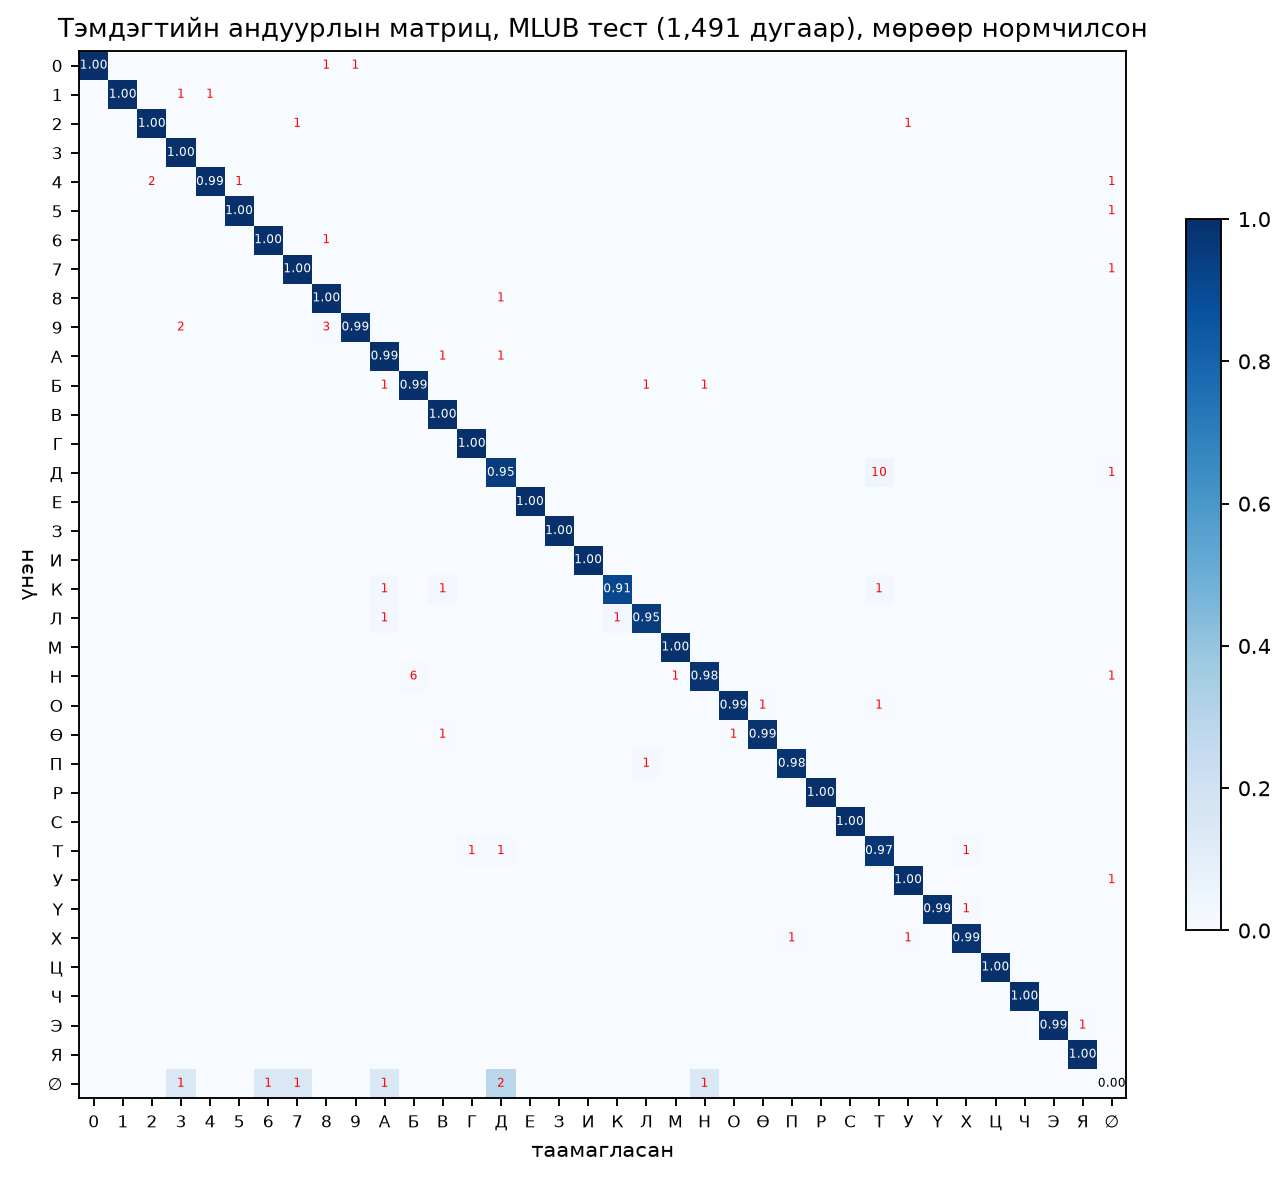
\includegraphics[width=0.92\textwidth]{confusion_mlub.png}
\caption{Тэмдэгтийн андуурлын матриц, MLUB тест (1\,491 дугаар, 10\,437 тэмдэгт), мөрөөр нормчилсон. Диагональд recall, диагоналиас гадуур алдааны тоо (улаан). $\varnothing$ нь орхигдсон (мөр) эсвэл илүү (багана) тэмдэгт.}\label{fig:cm}\end{figure}
\begin{figure}[H]\centering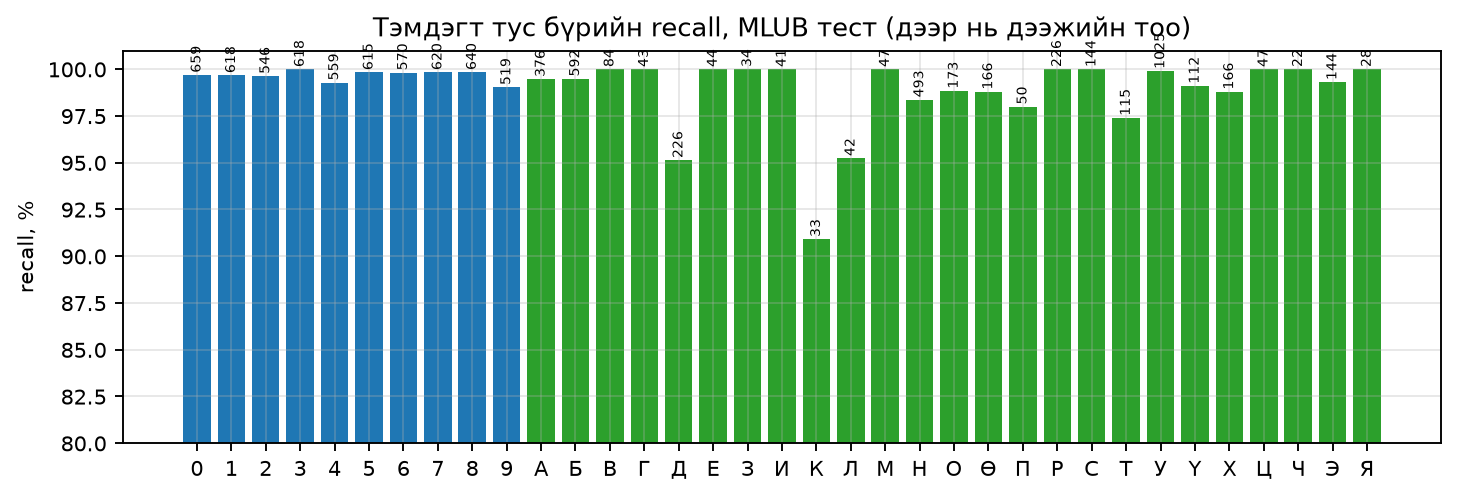
\includegraphics[width=\textwidth]{perchar_mlub.png}
\caption{Тэмдэгт тус бүрийн recall, MLUB тест; баганын дээр дээжийн тоо. Цэнхэр --- тоо, ногоон --- үсэг. Ховор серийн үсэг (К, Л, Д, Т) хамгийн бага.}\label{fig:perchar}\end{figure}
\begin{table}[H]\centering\caption{Хамгийн их андуурагдсан тэмдэгтийн хосууд, MLUB тест}\label{tab:conf}
\begin{tabular}{ccc|ccc}\toprule
Үнэн & Таамаг & Тоо & Үнэн & Таамаг & Тоо\\\midrule
Д & Т & 10 & Т & Х & 1\\
Н & Б & 6 & А & В & 1\\
9 & 8 & 3 & Т & Г & 1\\
9 & 3 & 2 & Ө & В & 1\\
4 & 2 & 2 & Э & Я & 1\\
$\varnothing$ & Д (илүү) & 2 & Ү & Х & 1\\\bottomrule
\end{tabular}\end{table}
\begin{figure}[H]\centering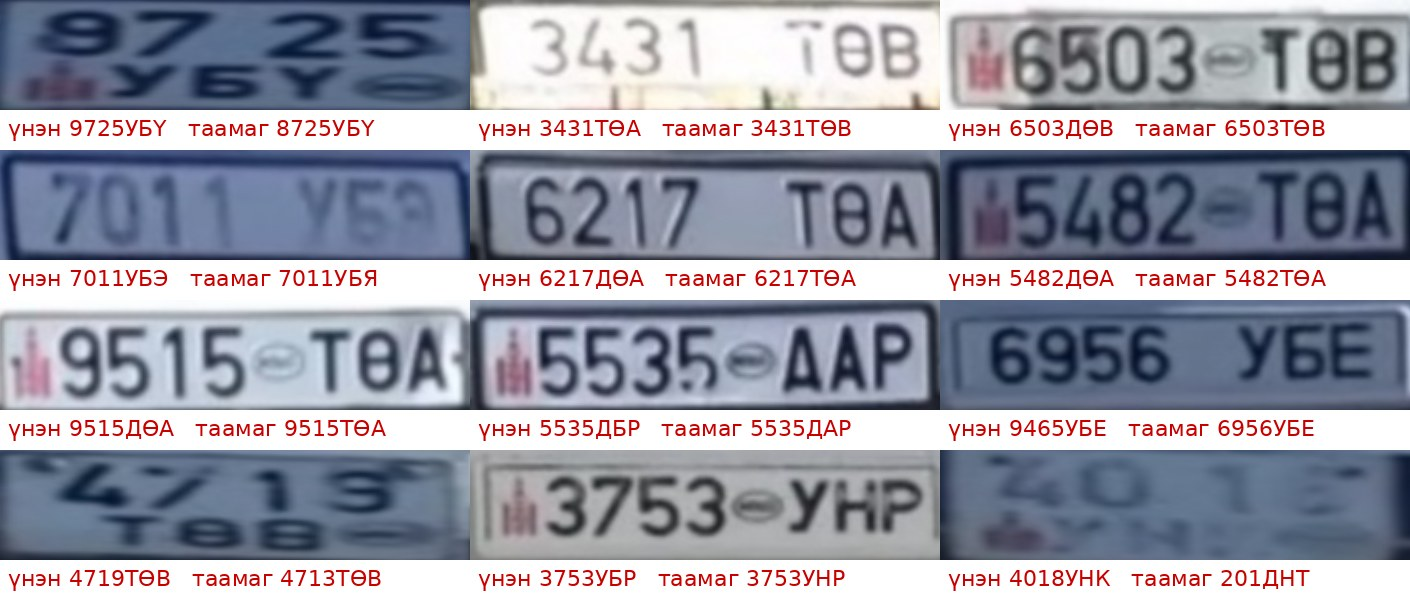
\includegraphics[width=\textwidth]{errors_mlub.jpg}
\caption{MLUB тест дээр буруу уншигдсан дугаарын жишээ (үнэн ба таамаг). Ихэнх нь бага нягтрал, бохирдол, хүчтэй шахалттай зураг дээрх нэг тэмдэгтийн андуурал.}\label{fig:errors}\end{figure}

\section{Төгсгөл хүртэлх үр дүн ба олон кадрын санал}
GitHub-ийн 18 бүтэн дүрстэй зураг (19 дугаар) дээр илрүүлэгч 18 дугаарыг IoU $\ge0.5$-аар олж (recall 94.7 хувь), 14-ийг яг зөв уншсан (73.7 хувь). Алдаа: нэг дугаар илрээгүй (\plate{2024УБЭ}); дөрөв нь сүүлийн үсгийн андуурал --- \plate{1537УНЛ}$\to$УНА, \plate{9494УБМ}$\to$УБИ, \plate{5947УБК}$\to$УБХ, \plate{3417УНТ}$\to$УНГ. Ижил 19 дугаарыг үнэн хайрцгаар өгөхөд 89.5 хувь байсан тул илрүүлэгчийн хайрцгийн зах, мөр хуваалтын зөрүү нэмэлт 2--3 алдаа үүсгэж байна. Зураг~\ref{fig:qual}-д төгсгөл хүртэлх жишээг үзүүлэв.
\begin{figure}[H]\centering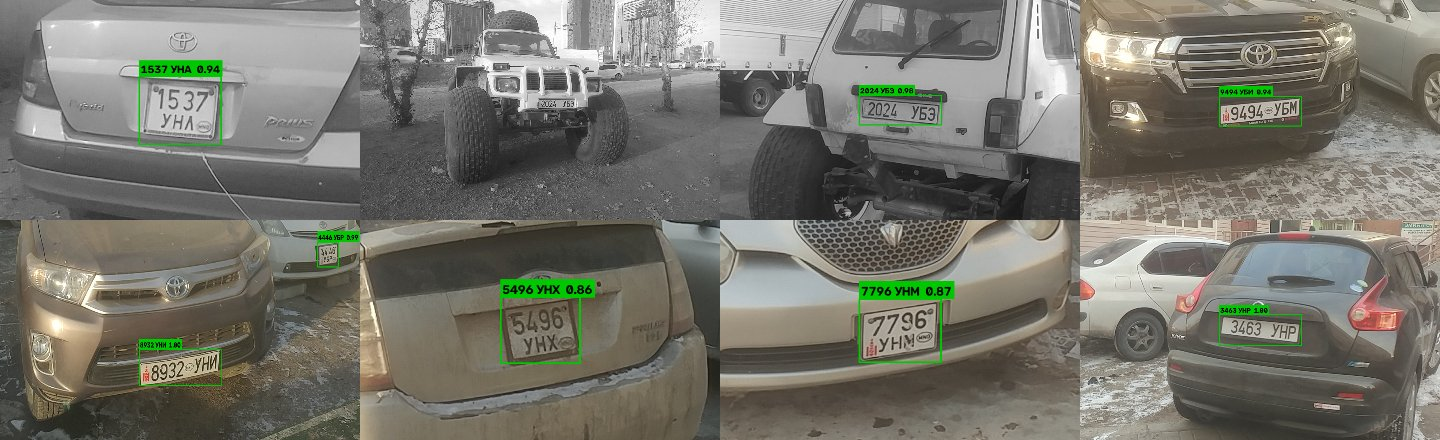
\includegraphics[width=\textwidth]{qualitative_github.jpg}
\caption{GitHub тестийн зураг дээрх төгсгөл хүртэлх үр дүн (ногоон: дүрэмд нийцсэн уншилт; шошго: дугаар ба уншигчийн итгэл). Нэг зурагт хоёр машин байхад хоёуланг нь олж уншсан жишээ.}\label{fig:qual}\end{figure}
Олон кадрын симуляцийн үр дүнг Зураг~\ref{fig:k}, Хүснэгт~\ref{tab:k}-д үзүүлэв. GitHub төгсгөл хүртэлх тестэд 3 кадрын санал 73.7-оос 78.9 хувь болгосон (нэг дугаар засагдсан), цаашид өсөөгүй; MLUB тайралтад санал 96.8 хувийг өөрчилсөнгүй. Учир нь симуляци нь нэг зургийн хувилбарууд дээр хийгдсэн тул алдаа \emph{системтэй} (бүх хувилбарт ижил тэмдэгт буруу) бөгөөд~\cite{wang2026mt}-д тэмдэглэснээр ийм алдааг санал засдаггүй. Бодит бичлэгт кадрууд өнцөг, зай, гэрлээр ялгаатай тул саналын ашиг тус илүү байхыг дараагийн хэсэг харуулна.
\begin{figure}[H]\centering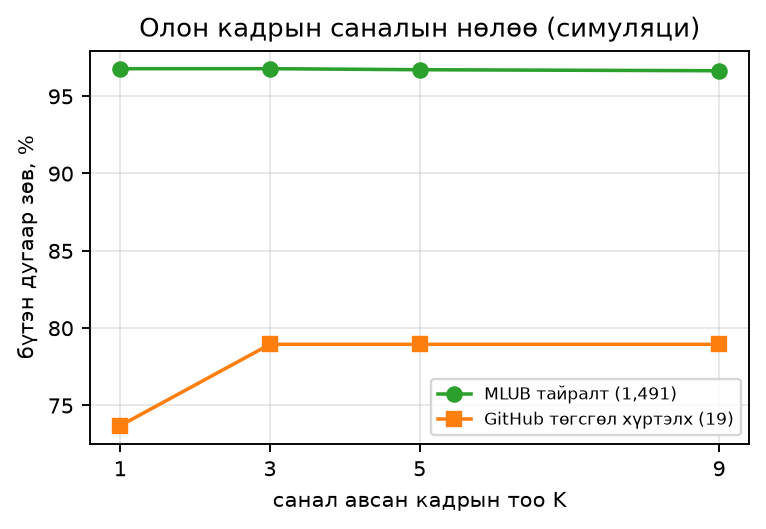
\includegraphics[width=0.6\textwidth]{multiframe_k.png}
\caption{Санал авсан кадрын тоо $K$-ийн нөлөө (симуляци).}\label{fig:k}\end{figure}
\begin{table}[H]\centering\caption{Олон кадрын саналын нөлөө, бүтэн дугаарын нарийвчлал (хувь), симуляцийн хувиргалт}\label{tab:k}
\begin{tabular}{lcccc}\toprule
Тест & $K=1$ & $K=3$ & $K=5$ & $K=9$\\\midrule
MLUB тайралт (1\,491) & 96.8 & 96.8 & 96.7 & 96.6\\
GitHub төгсгөл хүртэлх (19) & 73.7 & 78.9 & 78.9 & 78.9\\\bottomrule
\end{tabular}\end{table}

\section{Хугацааны хэмжилт}
Хүснэгт~\ref{tab:lat}, Зураг~\ref{fig:lat}-д 1920$\times$1080 кадрын боловсруулалтын хугацааг үзүүлэв. Нийт 7.3~мс (p95 9.8~мс) нь 100~мс зорилтоос 13 дахин бага бөгөөд 30~fps бичлэгийг бүх кадраар боловсруулах боломжтой. Анхны кадр 1.4~с (CUDA халаалт). GPU-гүй CPU дээр (16 цөм) 62~мс.
\begin{table}[H]\centering\caption{Нэг кадрын хугацаа, 1920$\times$1080, RTX 5080, FP16, 90 давталт (мс)}\label{tab:lat}
\begin{tabular}{lcccc}\toprule
Хэсэг & Дундаж & Медиан & p95 & Max\\\midrule
Илрүүлэгч (YOLO11n 640, урьд/дараах боловсруулалт орсон) & 4.0 & --- & --- & ---\\
Уншигч + дүрэм & 3.2 & --- & --- & ---\\
Нийт \texttt{process\_frame} & \textbf{7.3} & 7.0 & 9.8 & 12.8\\\bottomrule
\end{tabular}\end{table}
\begin{figure}[H]\centering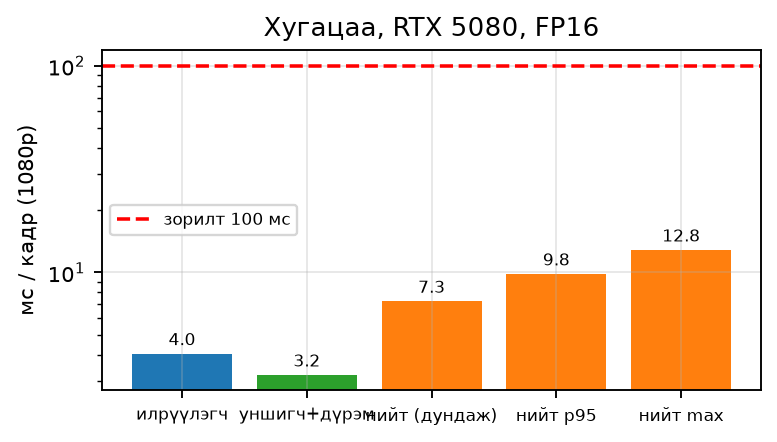
\includegraphics[width=0.6\textwidth]{latency.png}\caption{Хугацааны бүрэлдэхүүн (логарифм), 100~мс зорилттой харьцуулахад.}\label{fig:lat}\end{figure}

\section{Бичлэгийн туршилт}
Гурван бичлэгийг (хоёр нь гар утасны босоо 720$\times$1280, нэг нь хэвтээ 1280$\times$720, 30~fps) хоёр кадр тутамд нэгийг боловсруулж мөрдөлт, саналтайгаар ажиллуулав (Зураг~\ref{fig:video}, \ref{fig:tracks}). Нийт 29 мөр ($\ge3$ кадр) үүссэн. Хэвтээ, тогтвортой клипт 11 мөр бүгд дүрэмд нийцсэн дугаар өгч, margin 0.89--1.00, нэг кадрын санал нийцэл 0.30--1.00; нэг машин хоёр удаа орж ирэхэд ижил дугаар (\plate{1116 УНО}) гарсан. Гар утасны босоо клипт дугаар жижиг, хөдөлгөөний бүдэгтэй, налуу тул 18 мөрөөс 13 нь дүрэмд нийцсэн, 5 нь хог (хоёр зэргэлдээ дугаар нийлсэн зэрэг), санал нийцэл ихэвчлэн 0.3-аас бага. Үнэн шошго байхгүй тул энэ нь чанарын ажиглалт боловч margin ба санал нийцэл найдвартай/найдваргүй мөрийг тодорхой ялгаж байгаа нь хаалга нээх дүрэмд ашиглагдана.
\begin{figure}[H]\centering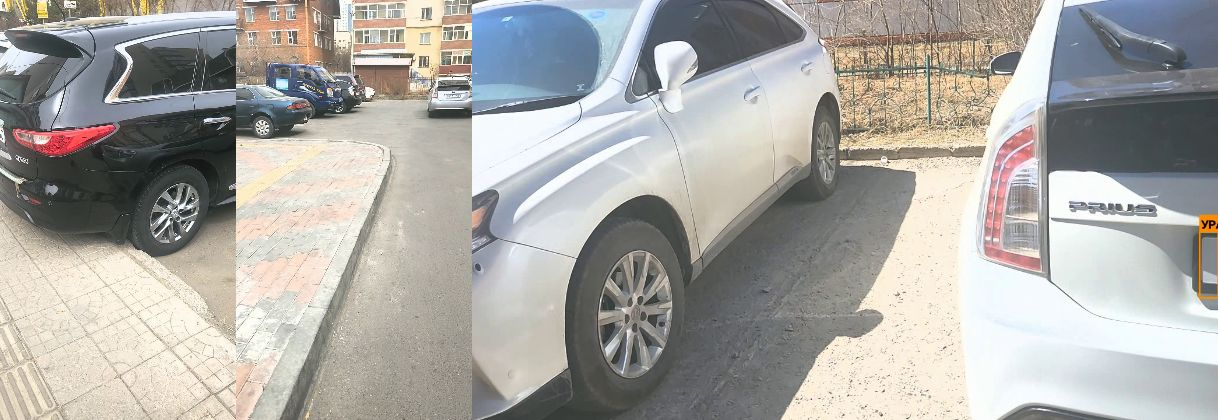
\includegraphics[width=\textwidth]{video_frames.jpg}
\caption{Гурван бичлэгийн тэмдэглэгээтэй кадр: мөр бүрийн санал нэгдсэн дугаар, итгэл, санал авсан кадрын тоо $n$.}\label{fig:video}\end{figure}
\begin{figure}[H]\centering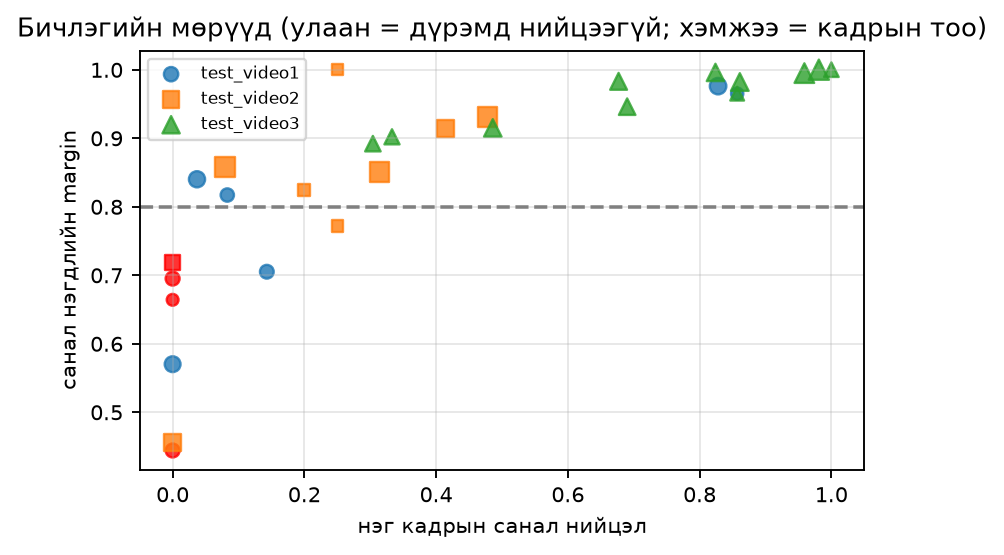
\includegraphics[width=0.7\textwidth]{video_tracks.png}
\caption{Бичлэгийн 29 мөр: нэг кадрын санал нийцэл ба санал нэгдлийн margin; улаан --- дүрэмд нийцээгүй; цэгийн хэмжээ --- кадрын тоо; тасархай шугам --- санал болгож буй margin босго 0.8.}\label{fig:tracks}\end{figure}

\section{Зорилттой харьцуулсан дүгнэлт}
\begin{table}[H]\centering\caption{Техникийн шаардлага ба хүрсэн үр дүн}\label{tab:targets}
\resizebox{\textwidth}{!}{\begin{tabular}{lccl}\toprule
Шаардлага & Зорилт & Хүрсэн & Байдал\\\midrule
Илрүүлэлт mAP$_{50}$ (монгол) & $\ge0.95$ & 0.992 & биелсэн\\
Бүтэн зөв уншилт, 1\,491 бодит дугаар & $\ge95$ хувь & 96.8 хувь (95 хувийн CI 96--98) & биелсэн\\
Хугацаа, 1080p кадр & $<100$~мс & 7.3~мс (p95 9.8) & биелсэн\\
Олон кадрын баталгаажуулалт & байх & IoU мөрдөлт + жинлэсэн санал & биелсэн\\
Төгсгөл хүртэлх, 19 бүтэн дүрстэй дугаар & $\ge95$ хувь & 73.7 / 78.9 хувь (CI 51--88) & биелээгүй\\
Туршилтын интерфэйс & байх & Gradio, зураг + бичлэг & биелсэн\\\bottomrule
\end{tabular}}\end{table}
